\documentclass[11pt,a4paper]{article}
\usepackage{gbstyle}
\begin{document}
\begin{center}
  {\sffamily\bfseries\LARGE GraphBudget}\\[5pt]
  {\sffamily\Large Deterministic Decode Optimization for SGLang}\\[8pt]
  {\color{GBGray}\small Technical Report \quad | \quad October 28, 2026}
\end{center}
\vspace{3mm}
\begin{center}
\begin{tabular}{ccc}
\GBmetric{+72.4\%}{median paired throughput gain} &
\GBmetric{5}{interleaved A/B pairs} &
\GBmetric{595}{GEMM and batch/reorder checks}\\
\end{tabular}
\end{center}
\vspace{2mm}
\begin{abstract}
GraphBudget studies deterministic decode performance at the SGLang execution boundary. The measurable result is an opt-in, small-$M$ BF16 GEMM specialization, adapted from the tile geometry proposed in SGLang PR \#42145. On an RTX 5070 Laptop GPU with Qwen2.5-0.5B-Instruct and a pinned SGLang v0.5.9 runtime, five interleaved paired serving runs show a median relative improvement of \textbf{72.4\%} in effective output throughput over the same configuration without the GEMM adaptation. Numerical checks and recorded kernel launches establish output equivalence and path activation within the tested conditions. This is a bounded performance result, not a general claim across engines, models or devices. Earlier CUDA Graph plan selection and decode-metadata candidates did not establish stable incremental throughput gains; those findings are preserved separately.
\end{abstract}

\Needspace{7\baselineskip}\section{Problem and contribution}
Decode often operates at small matrix-row counts. In the pinned deterministic SGLang path, the persistent Triton GEMM configuration uses larger output tiles than required by many decode-shaped calls. The work examines whether a guarded small-$M$ geometry can reduce serving cost without changing the deterministic arithmetic contract.

The measurable implementation consists of a source-pinned SGLang integration patch, an explicit selection guard, an opt-in GEMM geometry, numerical and request-level validation, and trace-based evidence. The kernel geometry is \emph{adapted} from bill-h-lin's upstream SGLang PR \#42145; it is not presented as a new GEMM algorithm or an upstream-merged change. The original GraphBudget capture-plan/cost-routing study is separate from the GEMM result.



\Needspace{7\baselineskip}\section{Implementation and numerical contract}
A guarded branch in \texttt{\_matmul\_persistent\_triton} specializes calls only if the explicit switch is enabled and the supported BF16, shape and stride requirements hold: $0<M\le16$, $K\bmod64=0$, $N\bmod128=0$, with required inner strides. Unsupported calls continue on the native route. For the selected configuration, the adaptation uses $B_M=16$, $B_N=64$, $B_K=128$, four warps and one program per output tile. The pinned GEMM's FP32 accumulation and fused-bias order remain unchanged.

The route is deliberately reversible. The patch neither introduces a new admission scheduler nor claims a general CUDA Graph recapture policy. Both the reference and candidate run under the same deterministic Triton backend and a fixed CUDA Graph configuration. This comparison isolates the local GEMM adaptation against its matched native route; it does not substitute for a comparison with contemporary fully tuned nondeterministic serving.

\begin{figure}[H]
\centering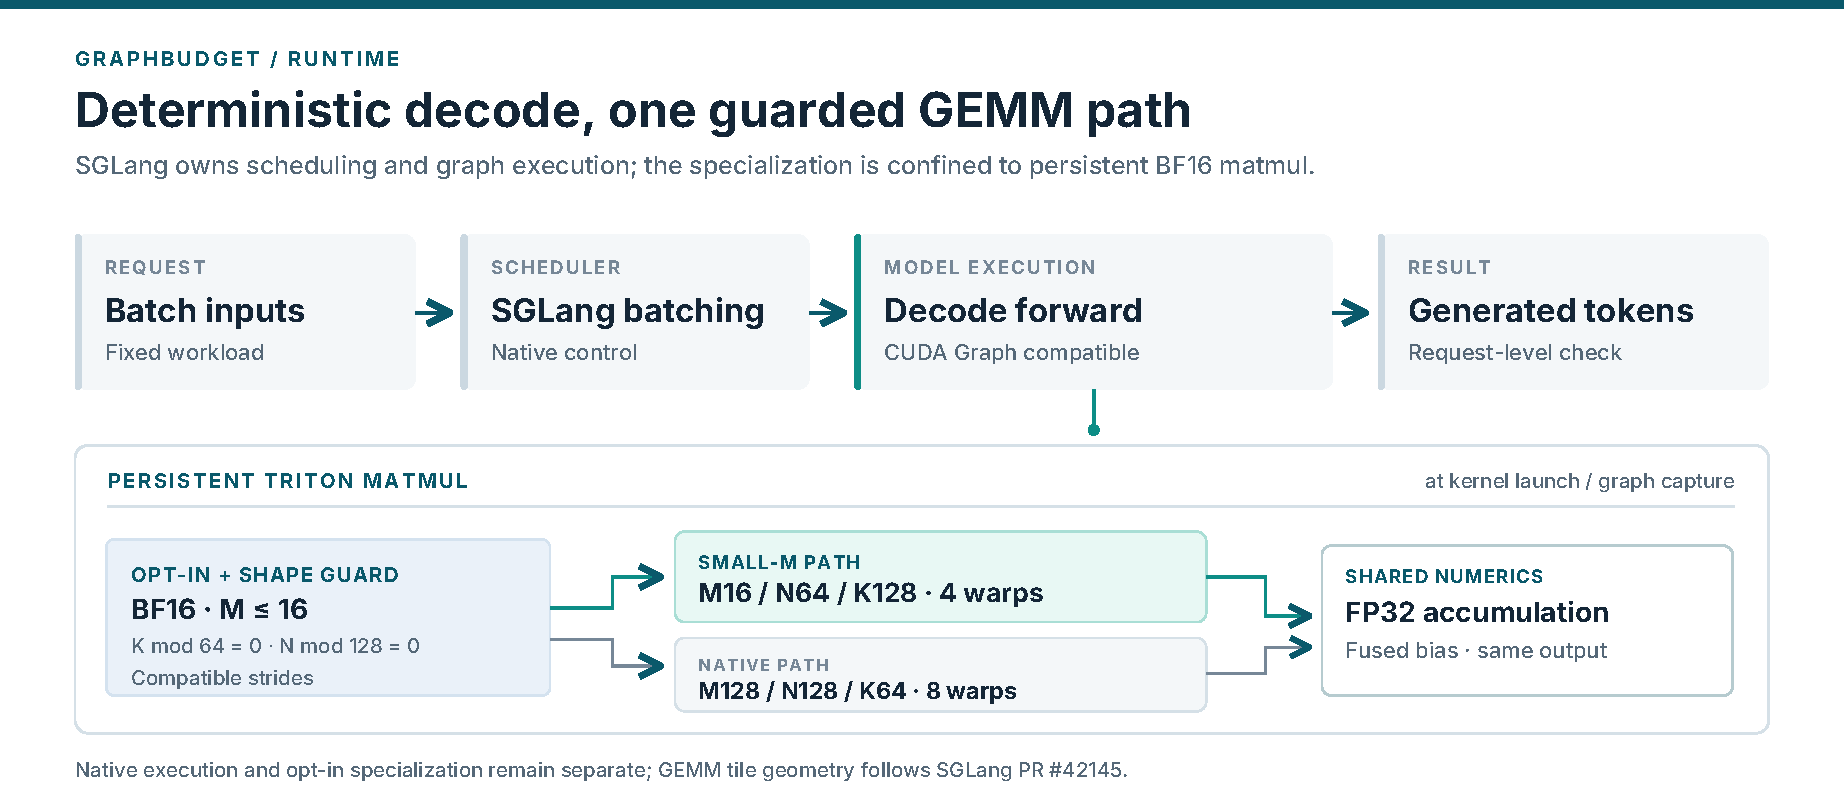
\includegraphics[width=\textwidth]{../figures/decode_architecture.pdf}
\caption{Execution boundaries and opt-in GEMM route. The selection is resolved when the kernel launch is prepared or captured; CUDA Graph replay uses its captured launch and does not dynamically redispatch on every output token.}
\end{figure}

\Needspace{16\baselineskip}\section{Experimental setup}
\begin{table}[H]\centering
\caption{Pinned workload and controls}\small
\begin{tabularx}{\textwidth}{@{}lX@{}}\toprule
Framework and GPU & SGLang v0.5.9 (base \texttt{bbe9c7e...}); NVIDIA RTX 5070 Laptop, WSL \\
Model & Qwen2.5-0.5B-Instruct, BF16, TP=1, greedy decode \\
Software & PyTorch 2.9.1+cu128; Triton 3.5.1; deterministic Triton attention/backend \\
Serving bounds & 16 maximum running requests; CUDA Graph capture sizes $[1,2,4,8,12,16]$; overlap disabled \\
Primary requests & 256 fixed requests, each producing 128 output tokens, in each experimental arm \\
Protocol & Five fresh-server interleaved pairs: AB, BA, AB, BA, AB \\
Metric & Effective output tokens per second; paired relative gain computed independently for each pair \\
\bottomrule
\end{tabularx}
\end{table}

\begin{figure}[H]
\centering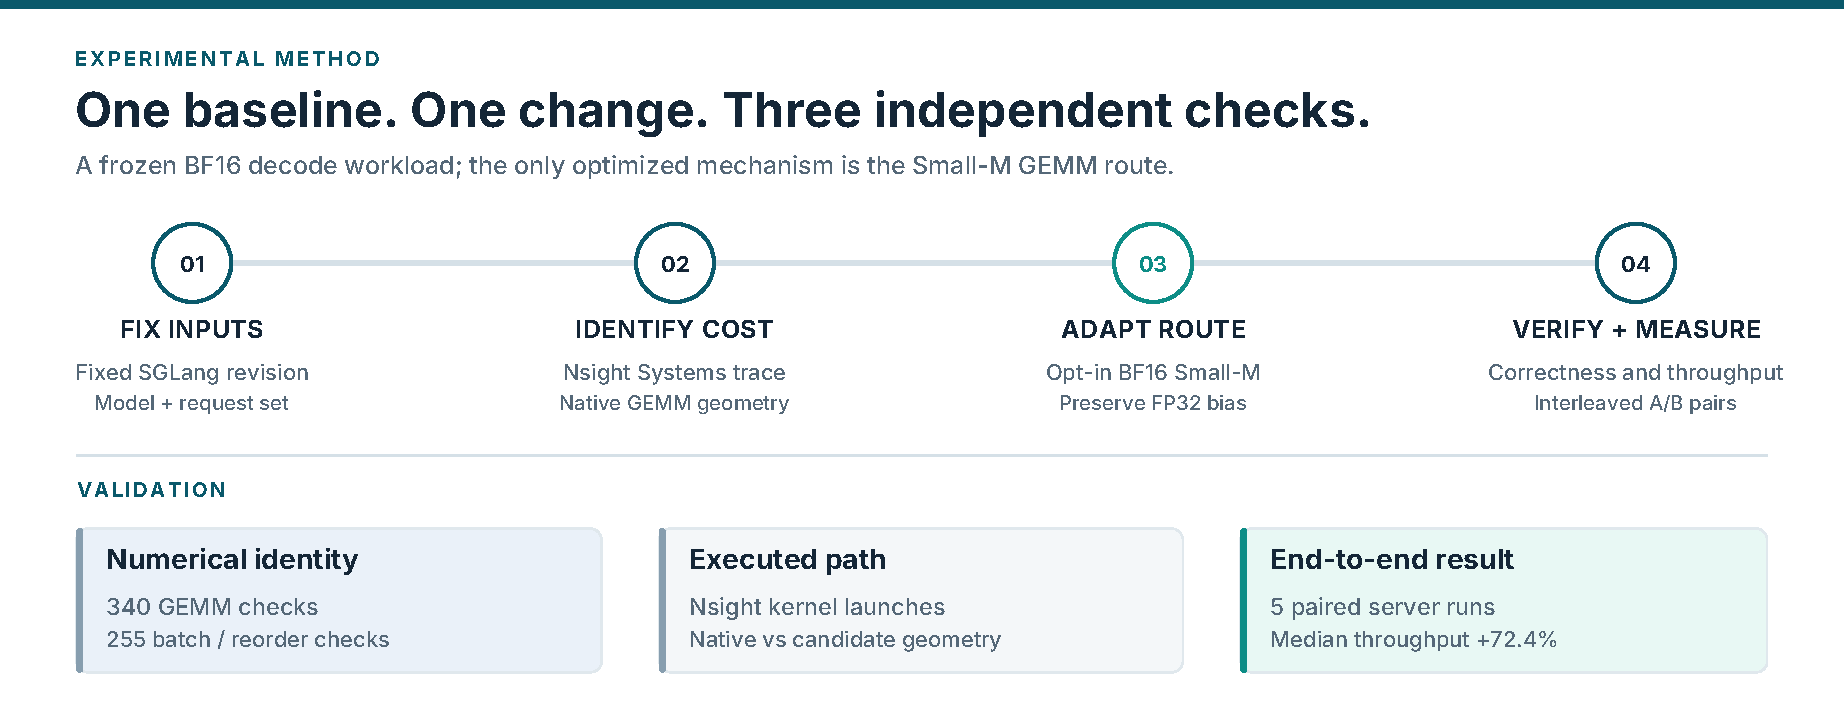
\includegraphics[width=\textwidth]{../figures/validation_workflow.pdf}
\caption{The validation sequence. Correctness checks precede the unprofiled request-level A/B comparison. Negative results are reported as distinct ablations.}
\end{figure}

\Needspace{7\baselineskip}\section{Serving performance}
\begin{table}[H]\centering
\caption{Five primary-load paired observations}\small
\begin{tabular}{@{}rrrr@{}}\toprule
Pair & Native (tokens/s) & Candidate (tokens/s) & Relative change \\\midrule
1 & 1,164.15 & 2,007.24 & +72.42\% \\
2 & 1,096.61 & 1,783.15 & +62.61\% \\
3 & 1,122.35 & 2,087.16 & +85.96\% \\
4 & 1,128.60 & 1,933.98 & +71.36\% \\
5 & 1,135.00 & 2,023.29 & +78.26\% \\\midrule
\multicolumn{3}{r}{Median of paired relative changes} & \textbf{+72.42\%}\\\bottomrule
\end{tabular}
\end{table}
\begin{figure}[H]
\centering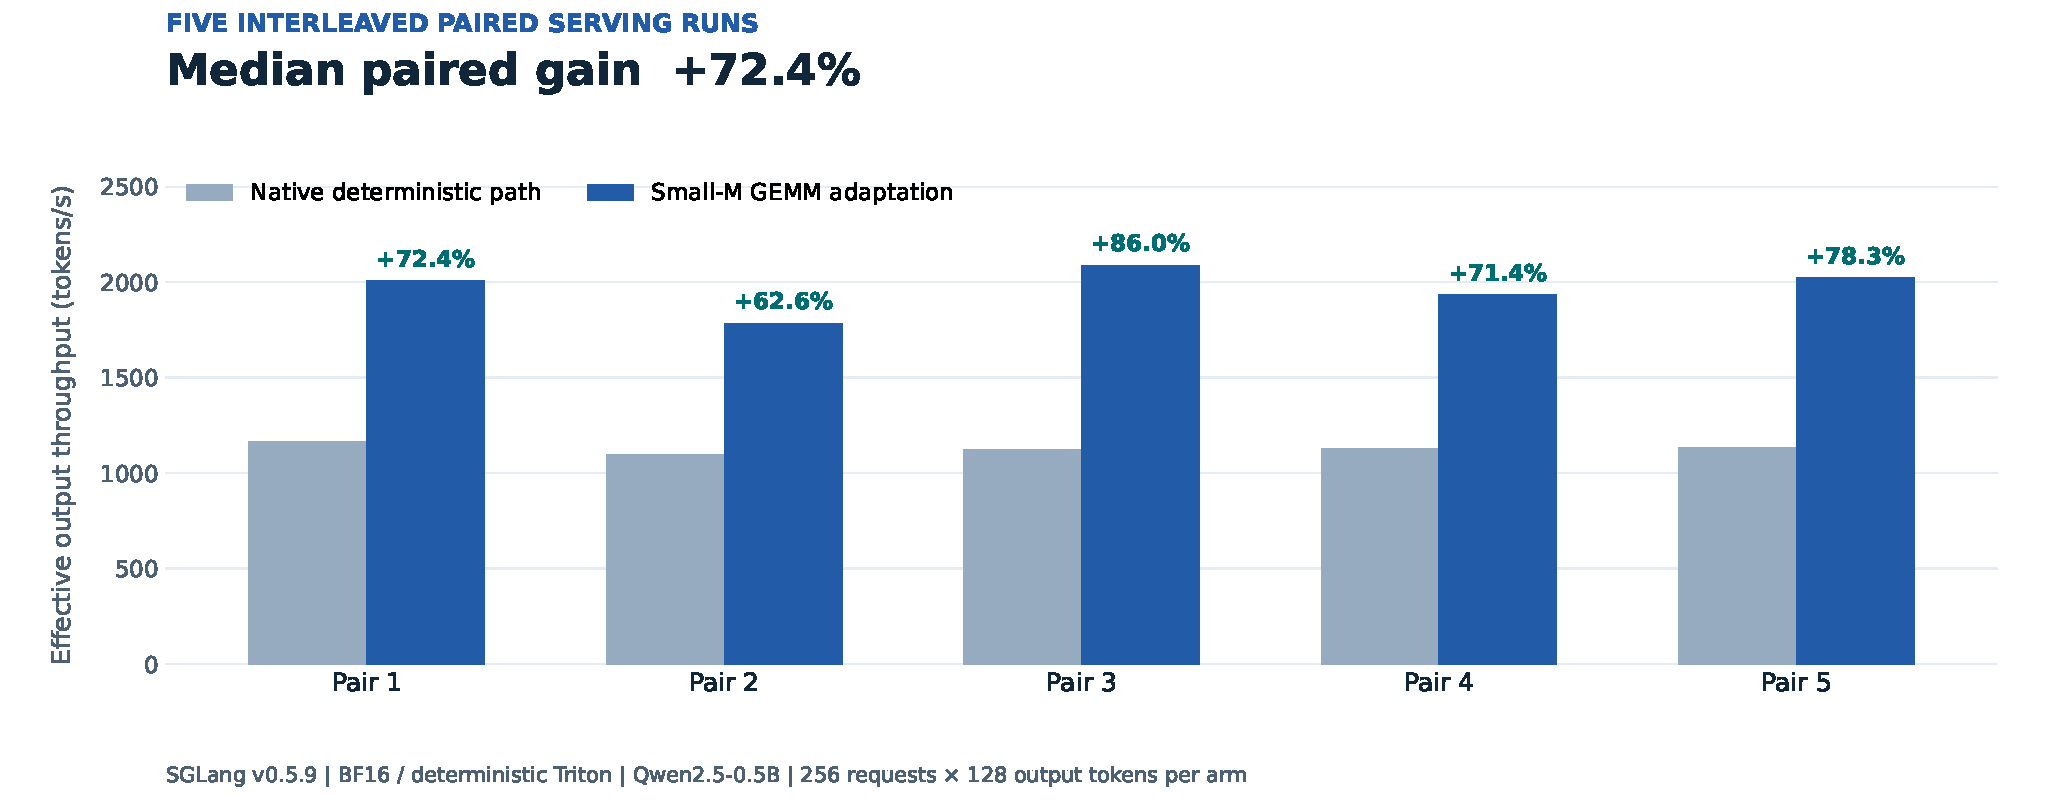
\includegraphics[width=\textwidth]{../figures/paired_throughput.pdf}
\caption{Effective output throughput per paired run, using the original deterministic Triton path as the comparator. Labels above the candidate bars show paired relative changes.}
\end{figure}
All five primary-load pairs are positive. Before/after A/A changes were +7.9\% and +8.8\%; these are two limited noise observations, not a confidence interval. The positive result is scoped to the measured fixed-workload configuration, not to arbitrary concurrent arrivals or other model families.

\Needspace{7\baselineskip}\section{Correctness and execution evidence}
The final loaded source passed 340 GEMM numerical checks across selected $M=1\ldots17$ and model-relevant matrix shapes; 170 of these used an independent exact CPU oracle. All 340 matched the native output bit for bit. An additional 255 checks exercised cross-batch reuse, row reordering and random bias. The measured request outputs were also token-identical across the tested arms. These tests establish the specified coverage only, not full mathematical equivalence for every supported tensor or device.

Nsight Systems recorded 63 CUDA Graph launches in each compared worker. Among 6,305 \texttt{matmul\_kernel\_persistent} activities, all native launches used 256 threads per block; the candidate used 128 threads for 6,113 activities and 256 for 192. This is direct evidence of a changed kernel launch path. The trace is diagnostic; the main throughput claim comes from the separate, unprofiled serving comparison.

\clearpage\section{Negative findings and interpretation}
\begin{table}[H]\centering\small
\caption{Ablations and measurement boundaries}\begin{tabularx}{\textwidth}{@{}p{.33\textwidth}X@{}}\toprule
Observation & Supported interpretation \\\midrule
Original CUDA Graph cost policy & No stable gain over the fair static configuration; native dispatch remains the preferred default. \\
Metadata preallocation & +0.8\% and $-1.0$\% in two comparison blocks; no established throughput improvement. \\
Metadata fusion & $-3.4$\% and $-6.1$\%; not adopted as a performance result. \\
Holdout TTFT & Mixed direction; median paired p50 change +21.5\% (worse). No general TTFT improvement claim. \\
GPU resource measurements & No established VRAM savings, KV expansion or cold-start acceleration. \\
Nsight Compute & Hardware counters unavailable (\texttt{ERR\_NVGPUCTRPERM}); no occupancy/bandwidth claim. \\
\bottomrule\end{tabularx}\end{table}
The negative findings reject two particular performance hypotheses; they do not invalidate the independently measured GEMM adaptation. They also set the boundary for the next research iteration: further work should first isolate a material hotspot and then measure an independent benefit beyond the current pinned path.

\Needspace{7\baselineskip}\section{Reproducibility and references}
The \href{https://github.com/yu830/graph-budget-runtime}{project repository} links to the fixed performance commit, SGLang source patch, structured paired-run statistics and exact environment instructions. The recorded software, model and workload identities are needed to reproduce the specific measurement. Partial or single-pair reruns do not constitute reproduction of all five accepted pairs.

\begin{enumerate}[leftmargin=1.6em,itemsep=.18em]
\item \href{https://github.com/sgl-project/sglang/pull/42145}{bill-h-lin, SGLang PR \#42145}, small-$M$ BF16 GEMM route and source geometry.
\item \href{https://github.com/yu830/graph-budget-runtime/blob/1f1984147608ee6c5dd8b3423e6f41877aaadeb4/docs/PERFORMANCE_RESULTS_20261027.md}{GraphBudget Performance Results}, fixed configuration, paired data and ablations.
\item \href{https://github.com/yu830/graph-budget-runtime/blob/1f1984147608ee6c5dd8b3423e6f41877aaadeb4/src/graphbudget/patches/sglang-v0.5.9.patch}{SGLang integration patch}, route, guards and runtime instrumentation.
\item \href{https://github.com/yu830/graph-budget-runtime/blob/1f1984147608ee6c5dd8b3423e6f41877aaadeb4/THIRD_PARTY_NOTICES.md}{Third-party notices}, retained provenance and licenses.
\end{enumerate}
\end{document}
